\documentclass[tikz,border=3pt]{standalone}
\usetikzlibrary{calc}

\begin{document}
    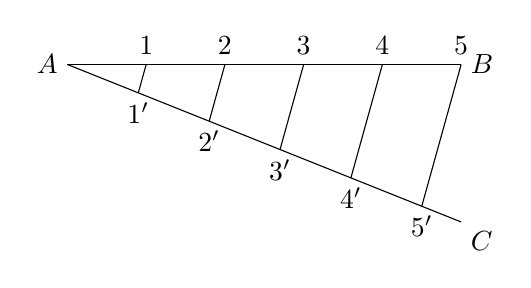
\begin{tikzpicture}[]
        % 标记点A, B, C
        \coordinate[label=left:{$A$}] (A) at (0,2);
        \coordinate[label=right:{$B$}] (B) at (5,2);
        \coordinate[label=below right:{$C$}] (C) at (5,0);

        % 绘制线段AB, AC
        \draw (A) -- (B);
        \draw (A) -- (C);

        % 等分线段AC
        \foreach \i in {1,2,...,5}
            {
                \coordinate[label=below:{$\i'$}] (a\i) at ($(A)!\i/5!(4.5,.2)$);
                \coordinate[label=above:{$\i$}] (b\i) at ($(A)!\i/5!(B)$);
                \draw (a\i) -- (b\i);
            }

    \end{tikzpicture}
\end{document}